\section{Биотический фон в сообществах {\it Macoma balthica}}
%из магистерской
Всего на исследованных участках нами было обнаружено $48$ таксонов беспозвоночных (таблица~\ref{tab:Barents_species}). 
При этом в пределах каждого из горизонтов литорали были встречены все таксоны. 
%		\begin{landscape}
\begin{footnotesize}
\begin{longtable}{|p{2cm}|p{0.4cm}p{0.4cm}|p{0.4cm}p{0.4cm}|p{0.4cm}p{0.4cm}|p{0.35cm}p{0.35cm}p{0.35cm}|p{1cm}|p{0.5cm}p{0.5cm}|p{1cm}|p{1cm}|}
\caption{Состав сообществ на исследованный участках литорали Баренцева моря}
\label{tab:Barents_species}
\\ \hline
участок                     & \multicolumn{2}{c|}{Абрам-мыс} & \multicolumn{2}{c|}{Пала-губа} & \multicolumn{2}{c|}{Гав\-ри\-ло\-во} & \multicolumn{3}{c|}{Яр\-ныш\-ная} & Дальне\-зе\-ле\-нец\-кая & \multicolumn{2}{c|}{Шель\-пи\-но} & Порч\-ни\-ха & Ива\-нов\-ская \\ \hline
горизонт литорали & С       & Н       & С       & Н       & С       & Н   & В    & С    & Н    & С           & В    & С    & С    & ВСЛ        \\ \hline \endfirsthead
	\hline
	\multicolumn{15}{|c|}{продолжение таблицы \ref{tab:Barents_species}} \\ \hline
участок                     & \multicolumn{2}{c|}{Абрам-мыс} & \multicolumn{2}{c|}{Пала-губа} & \multicolumn{2}{c|}{Гав\-ри\-ло\-во} & \multicolumn{3}{c|}{Яр\-ныш\-ная} & Дальне\-зе\-ле\-нец\-кая & \multicolumn{2}{c|}{Шель\-пи\-но} & Порч\-ни\-ха & Ива\-нов\-ская \\ \hline
горизонт литорали & С       & Н       & С       & Н       & С       & Н   & В    & С    & Н    & С           & В    & С    & С    & ВСЛ        \\ \hline
	\\ \hline \endhead
	\hline 
	\multicolumn{15}{|c|}{продолжение таблицы \ref{tab:Barents_species} на следующей странице}
	\\ \hline \endfoot
	 \endlastfoot
\multicolumn{15}{|c|}{Turbellaria} \\ \hline
 Turbellaria varia         &           &           &           &           &           &           &          &          &          &                 & +        & +        &          &            \\ \hline
\multicolumn{15}{|c|}{Nemertini} \\ \hline
Amphiporus lactiflorens   &           &           &           &           &           &           &          & +        &          &                 &          &          &          &            \\  \hline
Lineus gesserensis        &           &           & +         &           &           &           &          &          &          &                 &          &          & +        &            \\  \hline
Lineus ruber              &           &           &           &           &           &           &          &          &          &                 &          &          & +        &            \\  \hline
Nemertini varia           &           & +         &           &           & +         & +         & +        & +        &          & +               &          & +        & +        &            \\ \hline
\multicolumn{15}{|c|}{Priapulida} \\ \hline
Priapulus caudatus        &           &           &           & +         &           &           &          &          &          & +               &          &          & +        &            \\ \hline
\multicolumn{15}{|c|}{Oligochaeta} \\ \hline
Capitella capitata        & +         &           & +         & +         &           & +         &          &          &          & +               &          &          & +        &            \\  \hline
Enchytraeidae varia       &           &           & +         &           & +         & +         & +        &          & +        & +               & +        &          & +        &            \\  \hline
Nais sp.                  &           &           &           &           &           &           &          &          &          &                 & +        & +        &          &            \\  \hline
Oligochaeta gen. sp.      &           &           &           &           &           &           &          &          &          & +               &          &          &          &            \\  \hline
Paranais littoralis       &           &           &           &           &           &           &          & +        &          & +               &          &          &          &            \\  \hline
Tubifex costatus          & +         & +         & +         &           & +         &           &          & +        & +        & +               &          &          &          & +          \\  \hline
Tubificidae varia         & +         &           &           &           &           &           &          &          &          &                 &          &          &          &            \\  \hline
Tubificoides benedeni     &           &           & +         & +         & +         &           &          & +        &          & +               &          &          & +        & +          \\ \hline
\multicolumn{15}{|c|}{Polychaeta} \\ \hline
Alitta virens             &           & +         &           &           &           &           &          &          &          &                 &          &          &          &            \\  \hline
Arenicola marina          &           &           &           &           &           &           &          & +        &          & +               & +        & +        &          &            \\  \hline
Clitellio arenarius       &           & +         &           &           & +         & +         & +        & +        &          & +               &          & +        & +        &            \\  \hline
Eteone longa              &           &           & +         & +         &           &           &          &          &          &                 &          &          &          &            \\  \hline
Fabricia sabella          &           & +         & +         &           &           & +         & +        & +        &          & +               & +        & +        &          & +          \\  \hline
Nainereis quadricuspida   &           &           &           &           &           &           &          &          &          & +               &          &          & +        &            \\  \hline
Nereis pelagica           &           &           &           & +         &           &           &          &          &          &                 &          &          &          &            \\  \hline
Nereis sp.                &           &           & +         & +         &           &           &          &          &          &                 &          &          &          &            \\  \hline
Pectinaria koreni         &           &           &           & +         &           &           &          &          &          &                 &          &          &          &            \\  \hline
Phyllodoce groenlandica   &           &           &           & +         &           &           &          &          &          & +               &          &          &          &            \\  \hline
Polydora quadrilobata     &           &           &           &           &           &           &          &          & +        &                 &          &          &          &            \\  \hline
Pygospio elegans          & +         &           & +         & +         & +         & +         &          & +        &          & +               & +        & +        & +        &            \\  \hline
Sabellidae varia          &           &           & +         & +         &           &           &          &          &          &                 &          &          &          &            \\  \hline
Scalibregma infundibulum  &           &           &           &           &           &           &          &          & +        &                 &          &          &          &            \\  \hline
Scoloplos armiger         & +         &           &           &           & +         &           &          &          & +        & +               &          &          & +        &            \\  \hline
Spio sp.                  &           &           &           &           &           &           &          &          &          &                 &          &          &          & +          \\  \hline
Travisia forbesii         &           &           &           &           &           &           &          & +        & +        &                 &          &          &          &            \\ \hline
\multicolumn{15}{|c|}{Isopoda} \\ \hline
Jaera sp.                 &           &           &           &           &           &           &          & +        &          &                 & +        &          &          &            \\ \hline
\multicolumn{15}{|c|}{Amphipoda} \\ \hline
Gammarus sp.              & +         & +         & +         & +         &           &           & +        & +        &          & +               &          &          &          &            \\  \hline
Hyale prevosti            &           &           &           & +         &           &           &          &          &          &                 &          &          &          &            \\  \hline
Pseudolibrotus littoralis &           &           &           &           &           &           &          &          &          & +               &          &          &          &            \\ \hline
\multicolumn{15}{|c|}{Decapoda} \\ \hline
Crangon crangon           &           &           &           & +         &           &           &          &          &          &                 &          &          &          &            \\ \hline
\multicolumn{15}{|c|}{Diptera} \\ \hline
Chironomidae varia        & +         & +         &           & +         &           & +         & +        & +        & +        & +               & +        & +        & +        &            \\ \hline
\multicolumn{15}{|c|}{Gastropoda} \\ \hline
Epheria vincta            &           &           &           & +         &           &           &          &          &          &                 &          &          &          &            \\  \hline
Hydrobia ulvae            &           & +         & +         & +         &           &           &          & +        &          &                 &          &          & +        &            \\  \hline
Littorina gr. obtusata    &           &           &           &           &           &           &          &          &          &                 &          &          &          &            \\  \hline
Littorina gr. saxatilis   &           & +         & +         & +         &           &           &          & +        &          &                 & +        &          &          &            \\  \hline
Onoba aculeas             &           &           &           & +         &           &           &          & +        &          &                 &          &          &          &            \\  \hline
Skineopsis planorbis      &           &           &           &           &           &           &          & +        &          &                 &          &          &          &            \\ \hline
\multicolumn{15}{|c|}{Bivalvia} \\ \hline
Cerastoderma edule        &           &           & +         & +         &           &           &          & +        &          & +               &          &          & +        &            \\  \hline
Macoma balthica           & +         & +         & +         & +         & +         & +         & +        & +        & +        & +               & +        & +        & +        & +          \\  \hline
Mya arenaria              &           &           &           &           &           &           & +        & +        &          & +               &          &          & +        & +          \\  \hline
Mytilus edulis            & +         & +         & +         & +         & +         &           & +        & +        & +        & +               & +        & +        & +        &            \\  \hline
Turtonia minuta           &           &           &           &           &           &           &          &          &          &                 &          &          & +        &           \\ \hline

\end{longtable}
\end{footnotesize}
%\end{landscape}
Более трети таксонов ($17$ из $48$) - это редкие виды (встречены в одном описании), и лишь {\it Macoma balthica} встречается во всех описаниях. 
Количество таксонов на участке колебалось от $6$ (верхняя сублитораль губы Ивановская) до $22$ (средний горизонт литорали губы Дальнезеленецкая). 
По соотношению таксонов на всех участках преобладали Polychaeta.
	
Классификация участков по видовому составу была проведена при помощи кластеризации методом ближайшего соседа по коэффициенту Жаккара. 
Сходство по видовому составу чрезвычайно низко. 
Так, даже на уровне $50$\% сходства выделяется лишь две группы --- литораль губы Шельпино и средний горизонт литорали губ Дальнезеленецкая и Порчниха (рис.~\ref{ris:cluster_barents_species_tidal}). 
	\begin{figure}
		\begin{center}
			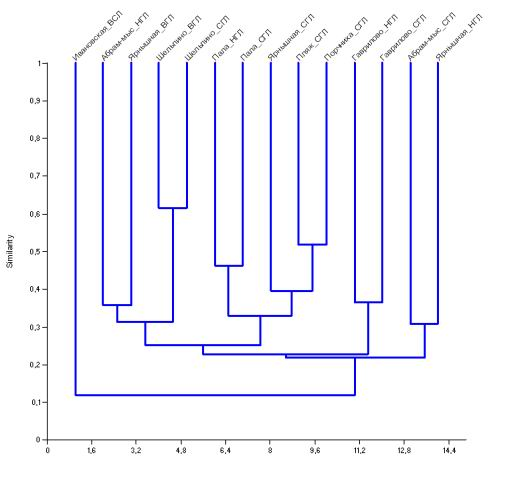
\includegraphics{../Barenc_Sea/soobshestvo/soobshestvo_po_gorizontam_Jakkard_paired_group_clusters.jpg}
		\end{center}
	\caption{Классификация отдельных горизонтов литорали по видовому составу}
	\label{ris:cluster_barents_species_tidal}

	\footnotesize{Кластеризация по методу ближайшего соседа с использованием коэффициента Жаккара. По оси ординат --- коэффициент Жаккара}
	\end{figure}
На еще более низком уровне сходства ($40$\%) выделяется литораль Пала-губы и губы Гаврилово. 

Возможно, что была выбрана слишком дробная единица анализа, и посмотрим как разложаться полные описания сообществ по изученных участкам литорали (рис.~\ref{ris:cluster_barents_species_sites}. 
	\begin{figure}
		\begin{center}
			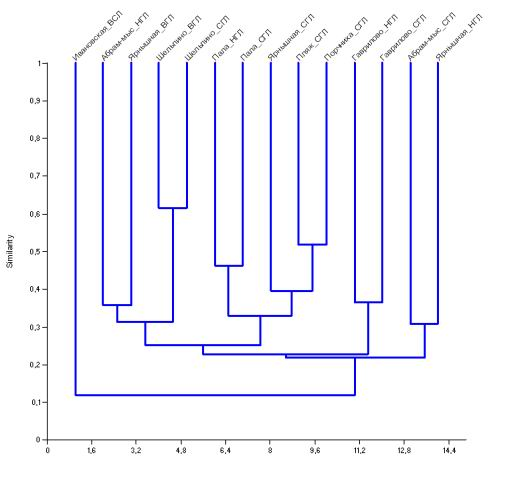
\includegraphics{../Barenc_Sea/soobshestvo/soobshestvo_po_gorizontam_Jakkard_paired_group_clusters.jpg}
		\end{center}
	\caption{Классификация участков по видовому составу}
	\label{ris:cluster_barents_species_sites}

	\footnotesize{Кластеризация по методу ближайшего соседа с использованием коэффициента Жаккара. По оси ординат --- коэффициент Жаккара}
	\end{figure}
На $50$\% уровне сходства было выделено одна группа участков --- губы Ярнышная, Дальнезеленецая и Порчниха.  
На более низком уровне сходства ($40$\%) к первой группе участков добавляется губа Гаврилово, и выделяется вторая группа сходных участков --- Абрам-мыс и губа Шельпино. 
Однако если в первой группе находятся участки, сближенные географически, то во вторую попали участки из разных акваторий.  

Влияние фактора гранулометрического состава грунта на состав сообщества было оценено с помощью анализа сходства ANOSIM. 
Градации фактора были заданы как илисто-песчаная, песчаная и гравийно-песчаная литораль, а в качестве меры сходства использовали коэффициент Жаккара. 
В результате не было обнаружено достоверного влияния данного показателя на видовой состав сообщества ($R=0,053, p=0,36$).
	
Таким образом, таксономический состав сообществ на исследованных участках достаточно вариабелен, и по-видимому, сходство определяется географической близостью участков. 

%была еще тема на конференции в Мурманске. Не надо ли добавить оттуда и пересчитать все нафиг.
